% Chapter Template

\chapter{Conclusiones} % Main chapter title

\label{Chapter5} % Change X to a consecutive number; for referencing this chapter elsewhere, use \ref{ChapterX}

En este capítulo se presentan las principales conclusiones del trabajo, así como también las futuras mejoras que se pueden realizar sobre el equipo.


\section{Conclusiones generales}

En la presente memoria se documentó el diseño e implementación de un Smart Plug. Se logró construir un prototipo funcional que permitió evaluar las prestaciones del equipo y desarrollar una aplicación para dispositivos móviles con sistema Android para poder interactuar con los Smart Plugs. 

La información provista por cada uno de los Plugs le permitirá al usuario conocer el consumo de los dispositivos eléctricos, ayudándolo a tomar decisiones con el objetivo de cambiar la forma en que los utiliza. Se tomó como principal objetivo en el diseño de la aplicación, que la misma fuera sencilla de utilizar y que presentara los datos de una forma útil.

Para la realización de este proyecto se aplicaron los conocimientos aprendidos en la carrera de especialización en sistemas embebidos, principalmente de las siguientes asignaturas:

\begin{itemize}
\item Arquitectura de microprocesadores: en la misma se aprendió la arquitectura del microcontrolador utilizado en el Smart Plug y técnicas básicas de programación. Fue la base para empezar a usar dichos microcontroladores.
\item Programación de microprocesadores: se aplicaron las metodologías aprendidas, el uso de capas para generar abstracción con el hardware y la teoría de programación orientada a objetos.
\item Ingeniería de software en sistemas embebidos: se aplicaron los conocimientos adquiridos para diseñar, implementar y probar tanto el firmware como la aplicación móvil.
\item Gestión de Proyectos en Ingeniería: lo aprendido en esta asignatura permitió abordar el proyecto de forma ordenada, previendo las tareas  que se debían realizar y el tiempo que se le debía dedicar a cada una de estas.
\item Sistemas Operativos de Tiempo Real: a pesar de que cuando se cursó esta materia, se enseñaba únicamente el uso de FreeRTOS, los conocimientos aprendidos permitieron entender, sin mayores dificultades, el uso de otro RTOS como es FreeOSEK.
\item Protocolos de comunicación en sistemas embebidos: se utilizó la comunicación SPI aprendida en la asignatura.
\item Diseño para manufacturabilidad: se discutieron los diseños y se realizaron revisiones y modificaciones para mejorar el funcionamiento del equipo.
\end{itemize}


Por otro lado, durante el desarrollo de este proyecto, se adquirieron conocimientos en las áreas de:

\begin{itemize}
\item Diseño de aplicaciones móviles: se aprendió la importancia del uso de maquetas al momento de diseñar una aplicación, lo cual facilita la articulación entre la estética buscada y la funcionalidad de la aplicación.
\item Programación de aplicación para el sistema Android: a pesar de que que se contaba con alguna experiencia en programación de aplicaciones bajo Android, la aplicación desarrollada introdujo el uso de nuevas clases, especialmente relacionadas con el manejo de servicios.
\end{itemize}


\section{Trabajo futuro}
\label{sec:trabajo_futuro}

\begin{figure}[!h]
	\centering
	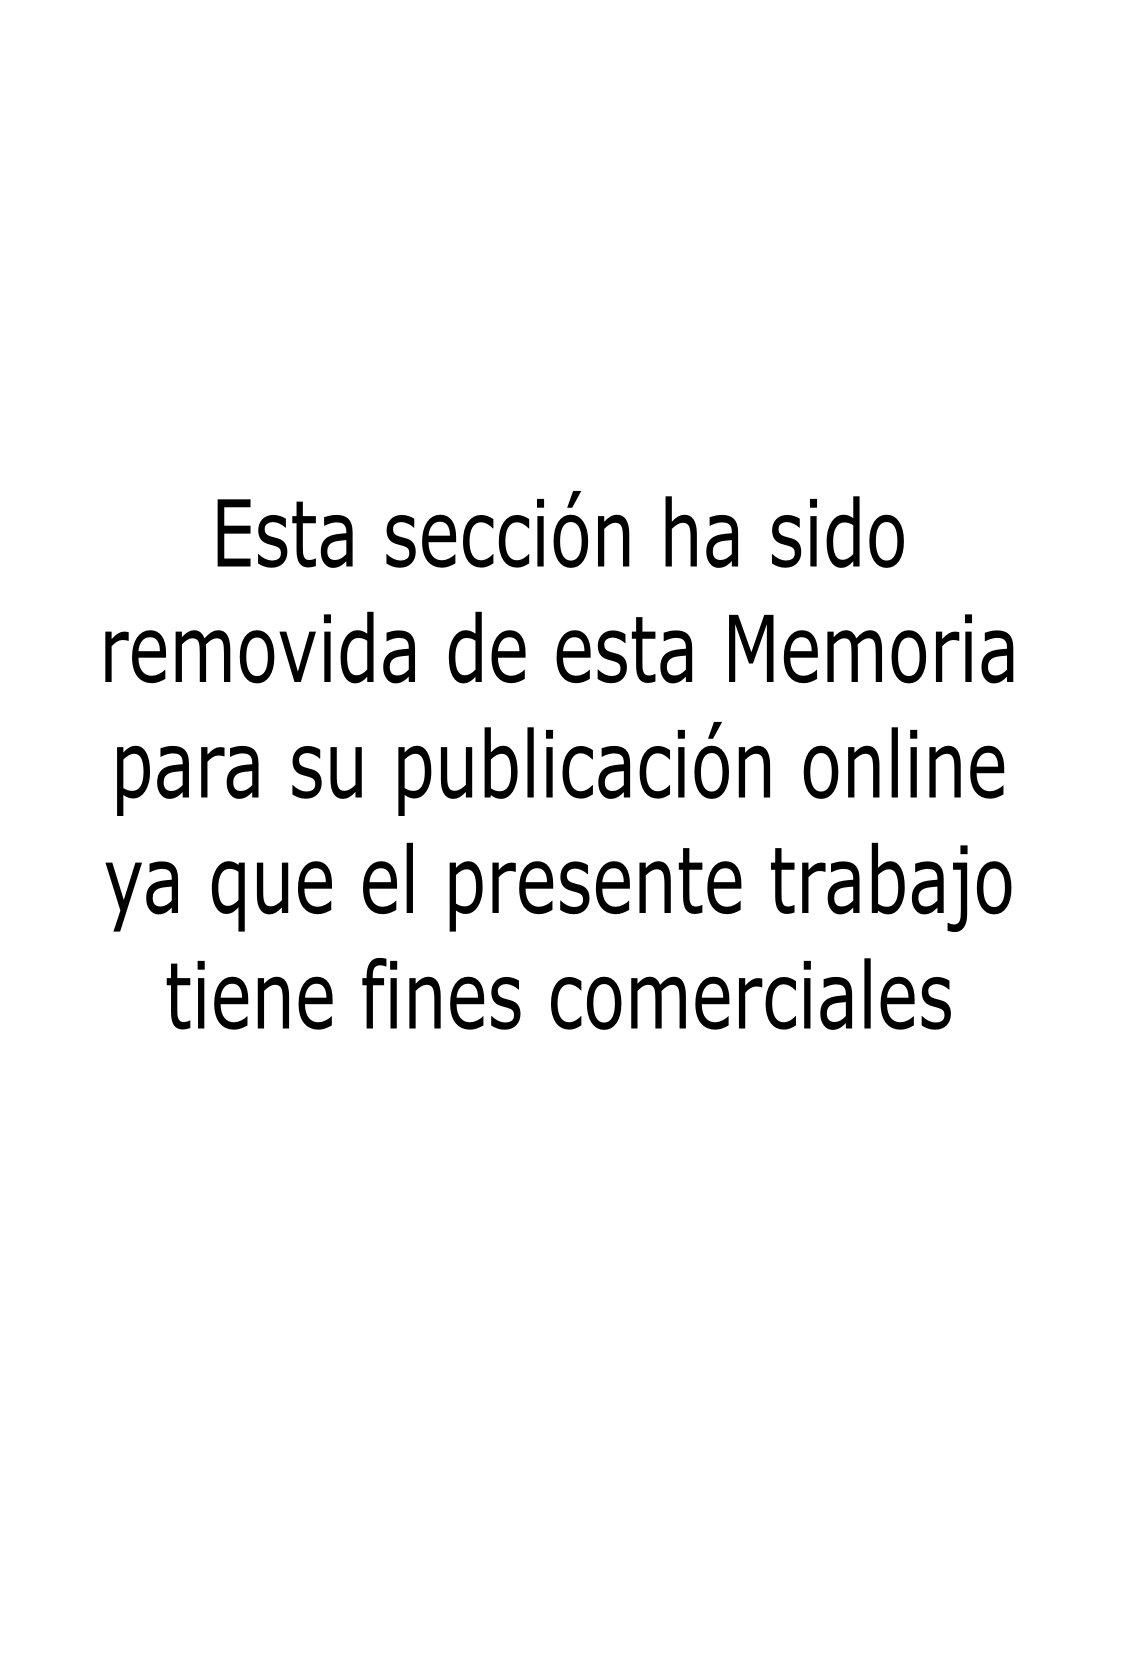
\includegraphics[width=14cm]{./Figures/comercial.png}
\end{figure}

